In this section, we discuss the performance of \pred\ with respect to an increasing horizon for each task $m\in [M]$. However, note that the number of tasks $\Mpr \geq n$.
%
% Finally, recall that when the horizon is small the weak demonstrator $\pi^w$ does not have sufficient samples for each action. This leads to a poor approximation of the greedy action. 
%
Note that \citet{lee2023supervised} studied linear bandit setting for $n=200$. We study the setting up to a similar horizon scale.


\textbf{Baselines:} We again implement the same baselines discussed in \Cref{sec:short-horizon}. The baselines are \pred, \predt, \dptg, \ad, \ts, and \linucb. 


\textbf{Outcomes:} We first discuss the main outcomes of our experimental results for increasing the horizon:

\begin{tcolorbox}
\customfinding \pred\ (\gt) outperforms \dptg, and \ad\ with increasing horizon.
\end{tcolorbox}

% \noindent
% \textbf{(1)} The \pred\ (\gt) learns to exploit the underlying latent structure and reward correlation between the different tasks even when $A \geq n$, $\Mpr \gg A$ with increasing horizon.

% \textbf{(2)} The \pred\ (\gt) outperforms its weak demonstrator even when trained on $\Htr\subseteq\Dpr$.



% \textbf{(3)} The \pred\ outperforms \dptg\ 

% performance drops for a more complex non-linear feedback setting with an increasing number of dimensions.



% \begin{figure}[!hbt]
% \centering
% \begin{tabular}{ccc}
% \subfigure[Horizon $20$]{\hspace*{-1.5em}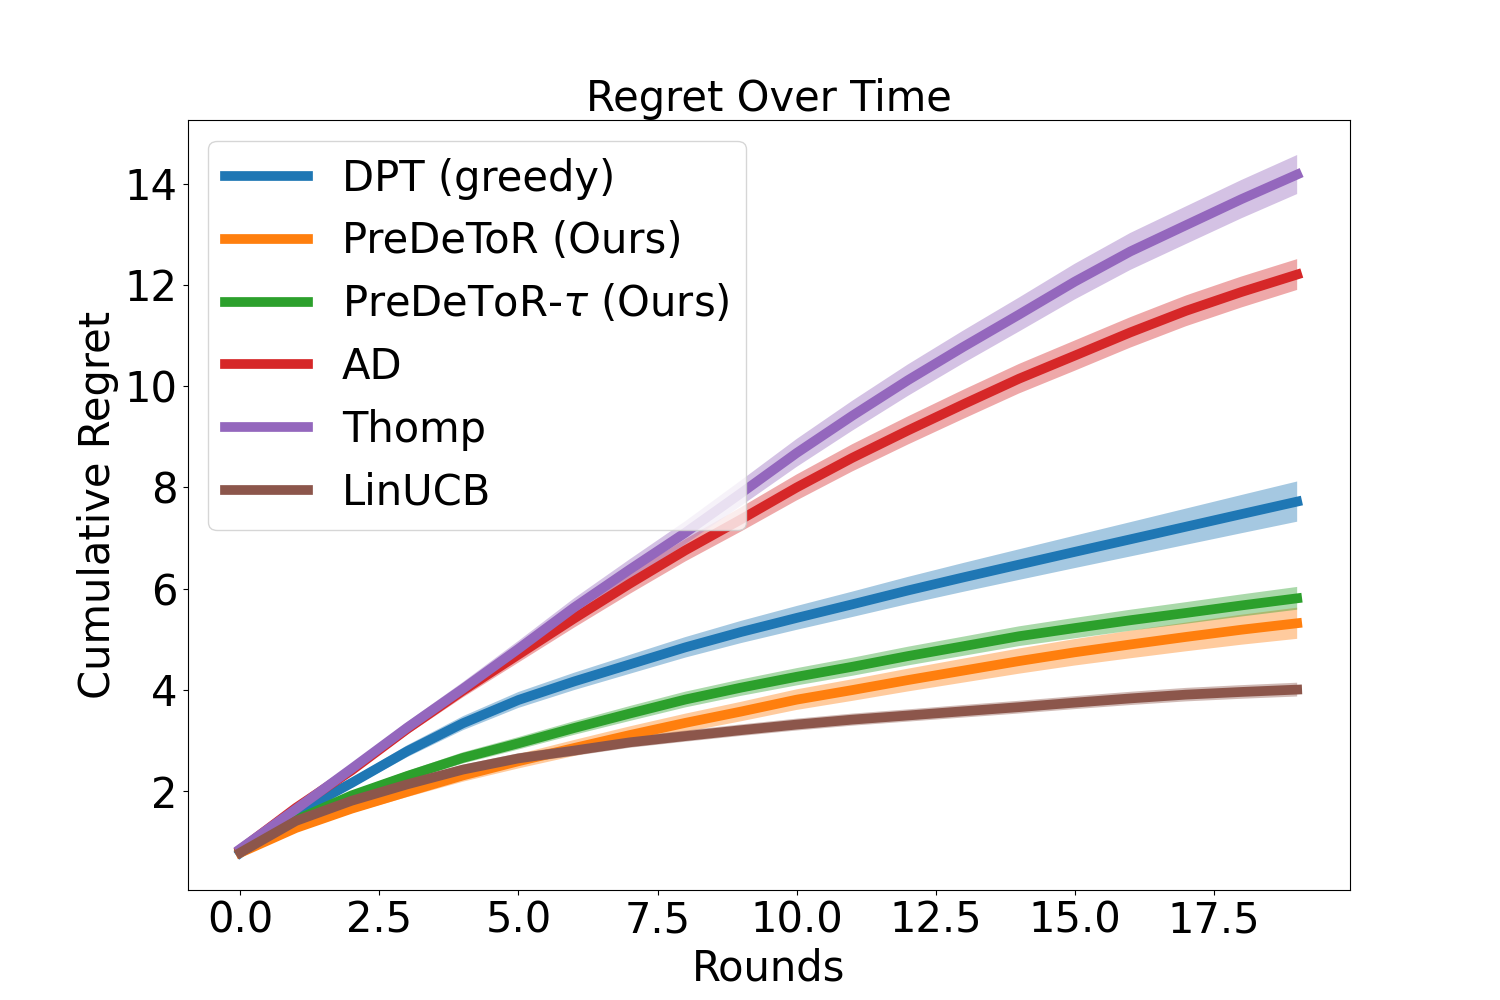
\includegraphics[scale = 0.13]{img/Neurips/horizon/lin_H20_lr0.00015_do0_embd32_layer4_head4_envs150080_hists1_samples1_var0.3_cov0.0_H20_d20_lind5_seed1_testcov0.0_hor20.pkl.png}\label{fig:hor-20}} &
% %%%%%%%%%%
% \hspace*{-1.5em}\subfigure[Horizon $40$]{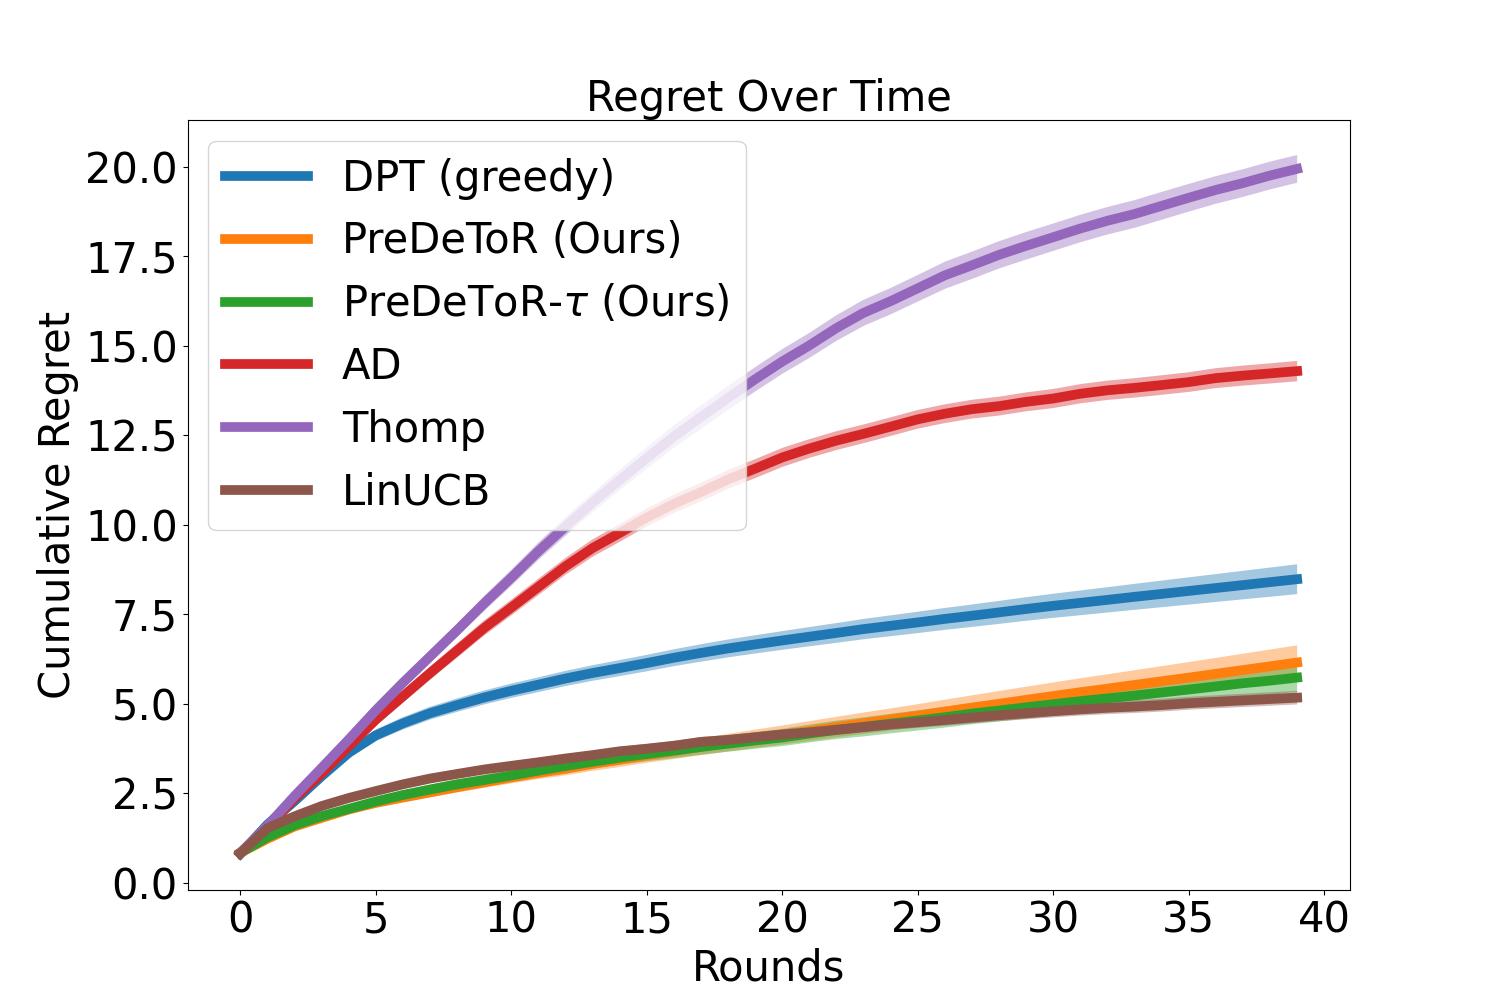
\includegraphics[scale = 0.13]{img/Neurips/horizon/lin_H40_lr0.00015_do0_embd32_layer4_head4_envs150080_hists1_samples1_var0.3_cov0.0_H40_d20_lind5_seed1_testcov0.0_hor40.pkl.png} \label{fig:hor-40}} &
% %%%%%%%%%%%%%%%%%%%%%%%
% \subfigure[Horizon $60$]{\hspace*{-1.5em}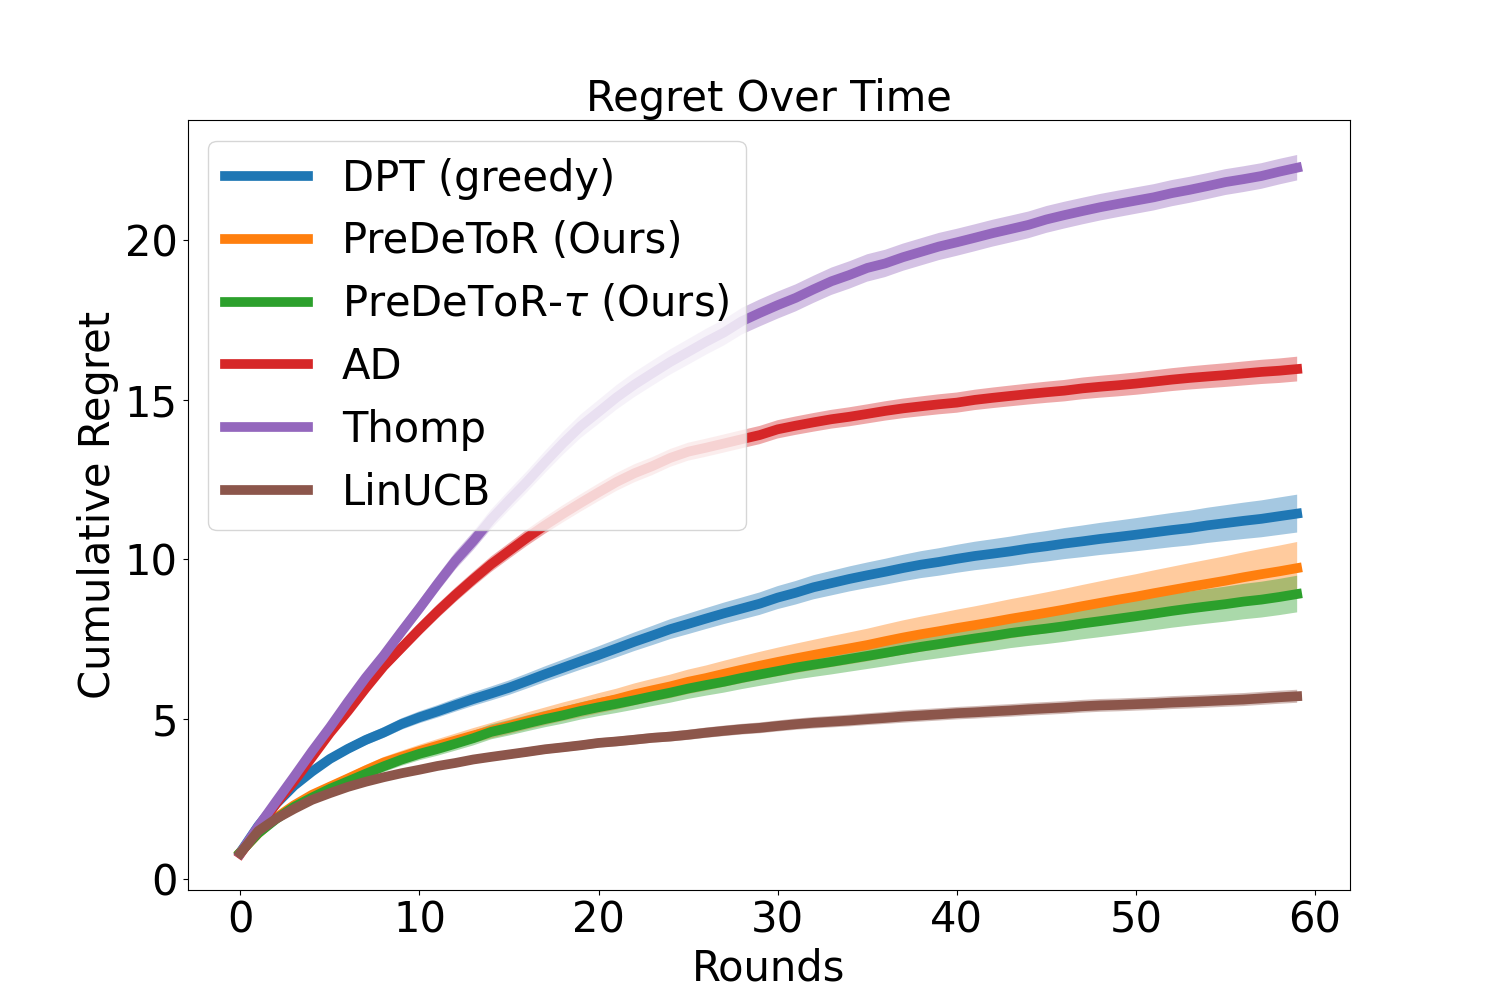
\includegraphics[scale = 0.13]{img/Neurips/horizon/lin_H60_lr0.00015_do0_embd32_layer4_head4_envs150080_hists1_samples1_var0.3_cov0.0_H60_d20_lind5_seed1_testcov0.0_hor60.pkl.png}\label{fig:hor-60}} \\
% %%%%%%%%%%%%%%%%%
% %%%%%%%%%%%%%%%%%%%
% \hspace*{-1.5em}\subfigure[Horizon $100$]{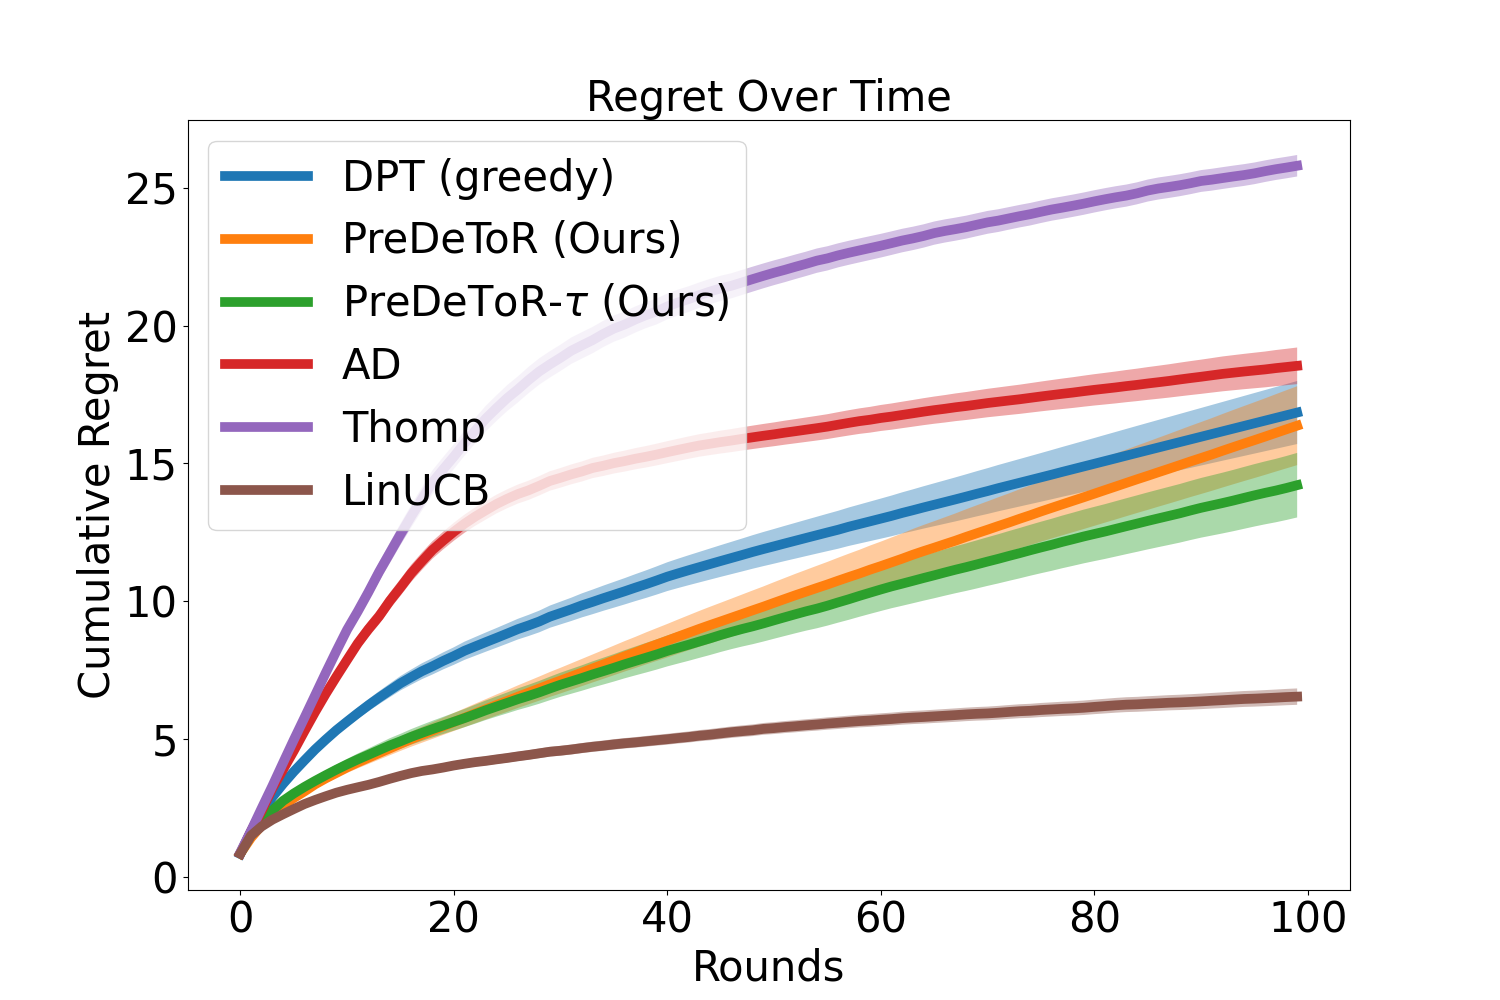
\includegraphics[scale = 0.13]{img/Neurips/horizon/lin_H100_lr0.00015_do0_embd32_layer4_head4_envs150080_hists1_samples1_var0.3_cov0.0_H100_d20_lind5_seed1_testcov0.0_hor100.pkl.png} \label{fig:hor-100}} &
% %%%%%%%%%%%%%%%%%%%%%%%%%%%%%%%%
% \hspace*{-1.5em}\subfigure[Horizon $120$]{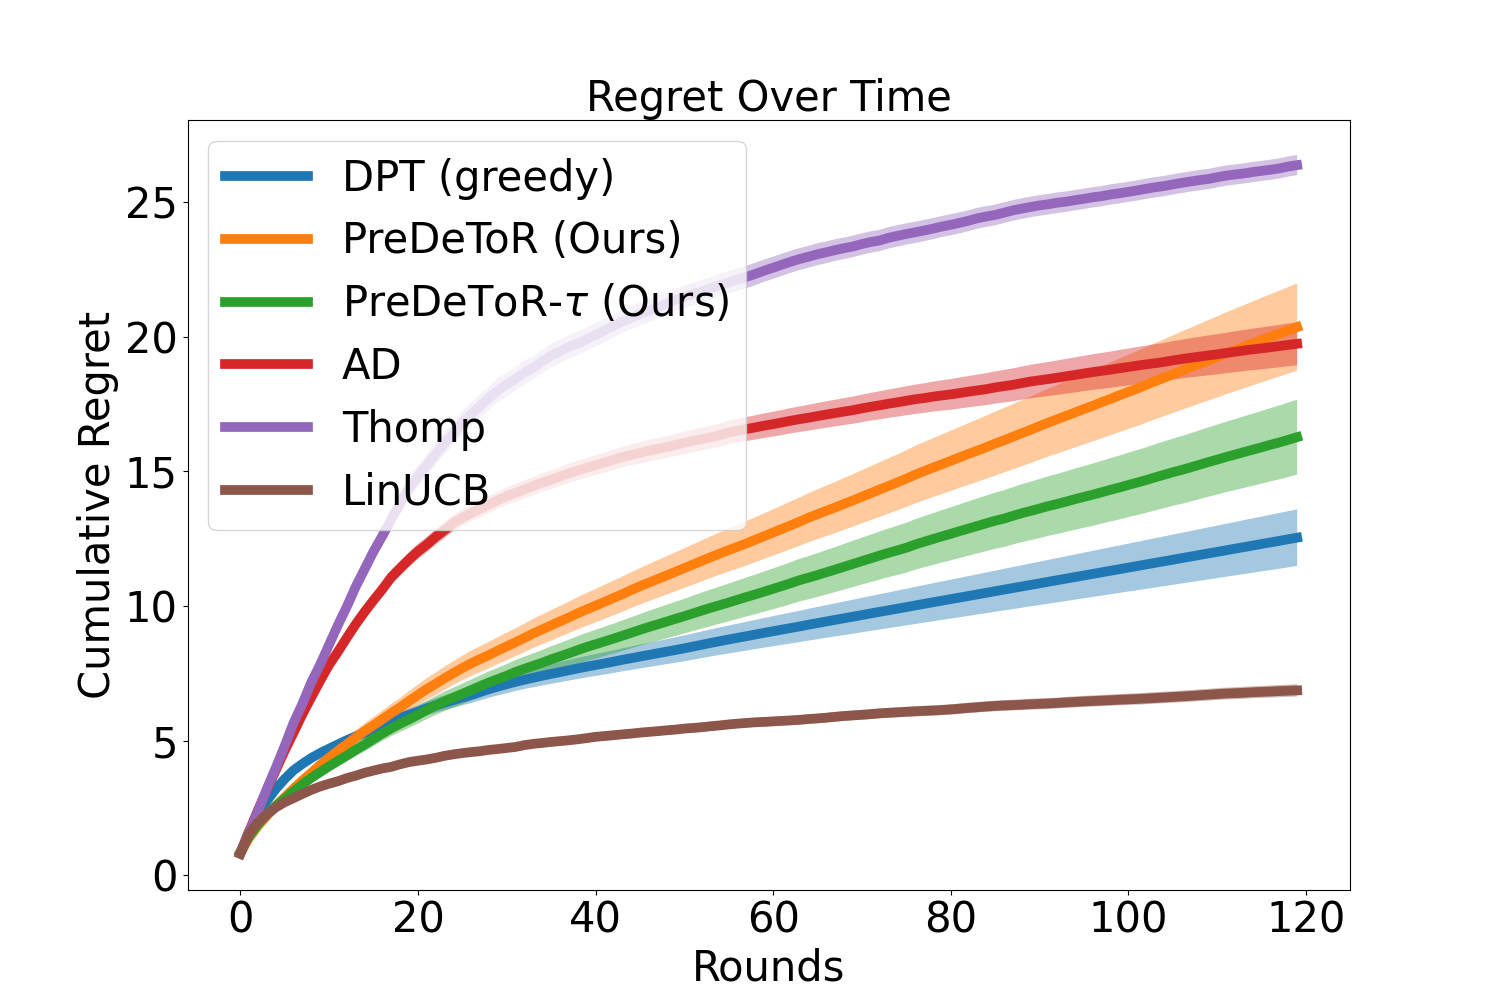
\includegraphics[scale = 0.13]{img/Neurips/horizon/lin_H120_lr0.00015_do0_embd32_layer4_head4_envs150080_hists1_samples1_var0.3_cov0.0_H120_d20_lind5_seed1_testcov0.0_hor120.pkl.png} \label{fig:hor-120}} &
% %%%%%%%%%%%%%%%%%%%%%%%%%%%%%%
% \hspace*{-1.5em}\subfigure[Horizon $140$]{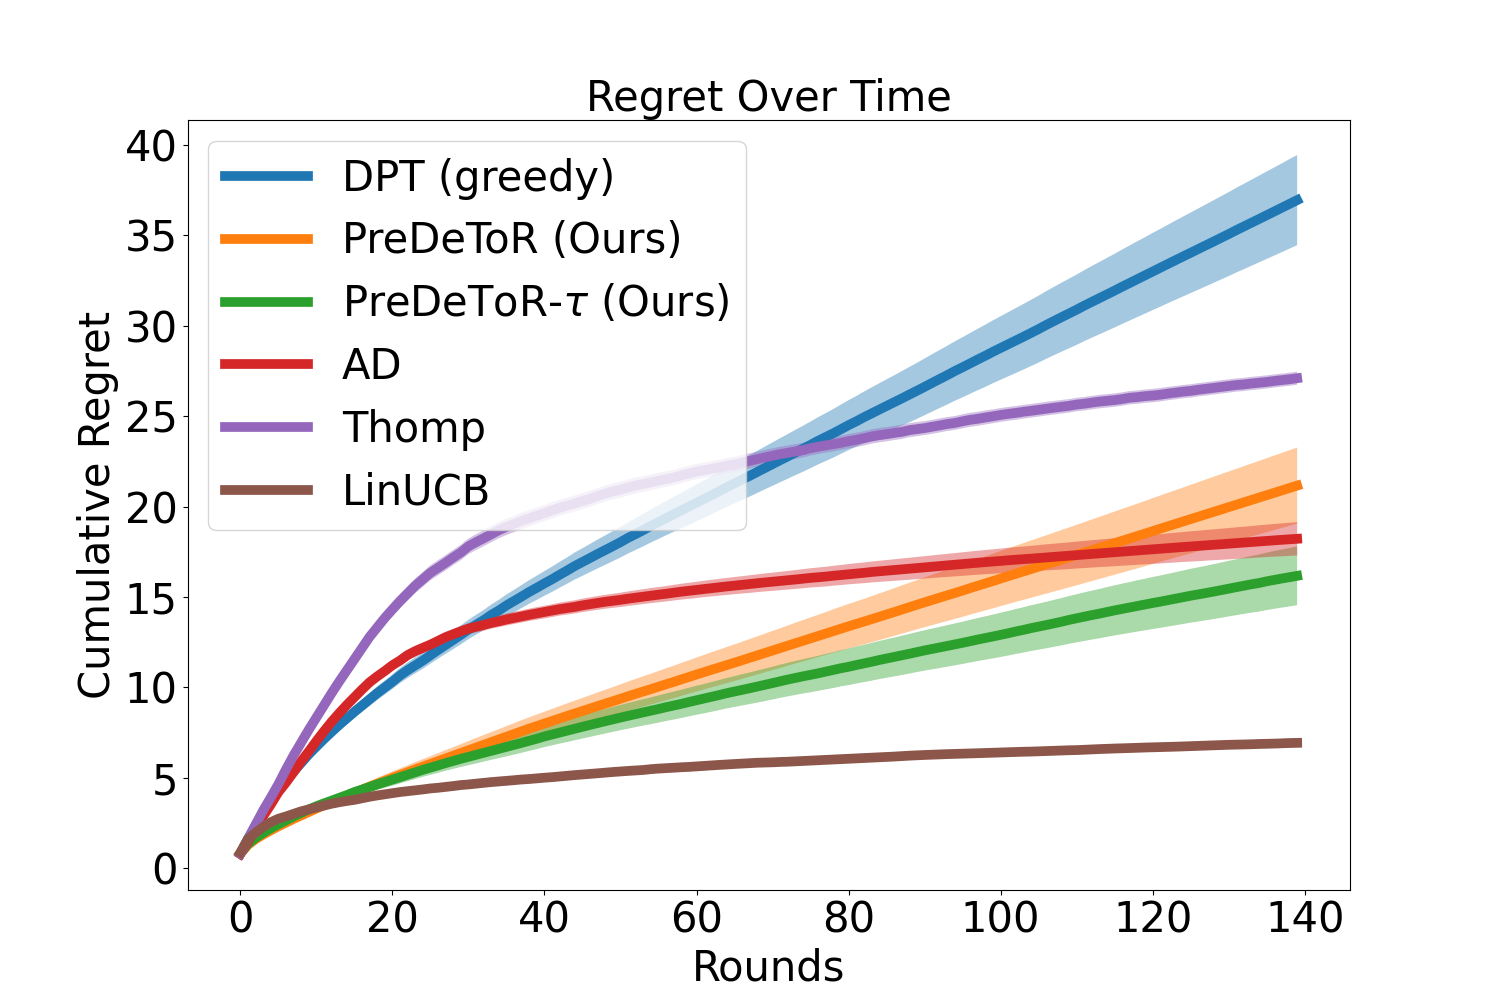
\includegraphics[scale = 0.13]{img/Neurips/horizon/lin_H140_lr0.00015_do0_embd32_layer4_head4_envs150080_hists1_samples1_var0.3_cov0.0_H140_d20_lind5_seed1_testcov0.0_hor140.pkl.png} \label{fig:hor-140}} %\\
% %%%%%%%%%%%%%%%%%%%%%%%%%%%%%%%
% \end{tabular}
% \begin{tabular}{cc}
% \hspace*{-1.5em}\subfigure[Horizon $200$]{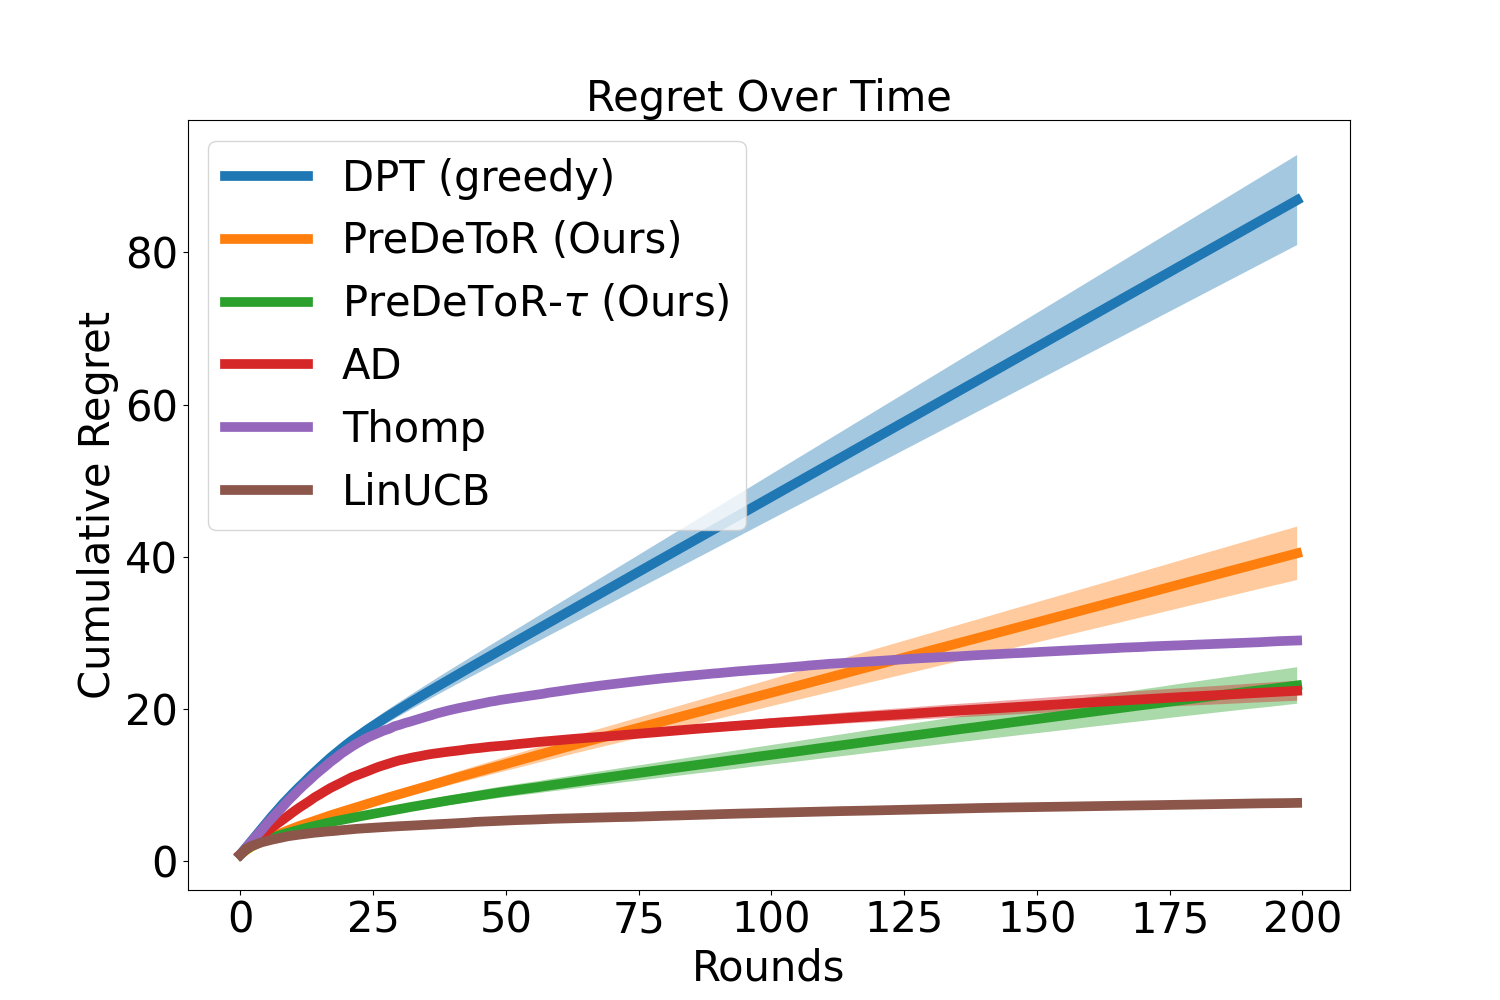
\includegraphics[scale = 0.13]{img/Neurips/horizon/lin_H200_lr0.00015_do0_embd32_layer4_head4_envs150080_hists1_samples1_var0.3_cov0.0_H200_d20_lind5_seed1_testcov0.0_hor200.pkl.png} \label{fig:hor-200}} &
% % %%%%%%%%%%%%%%%%%%%%%%%%%%%%%%%
% \hspace*{-1.5em}\subfigure[Increasing Horizon]{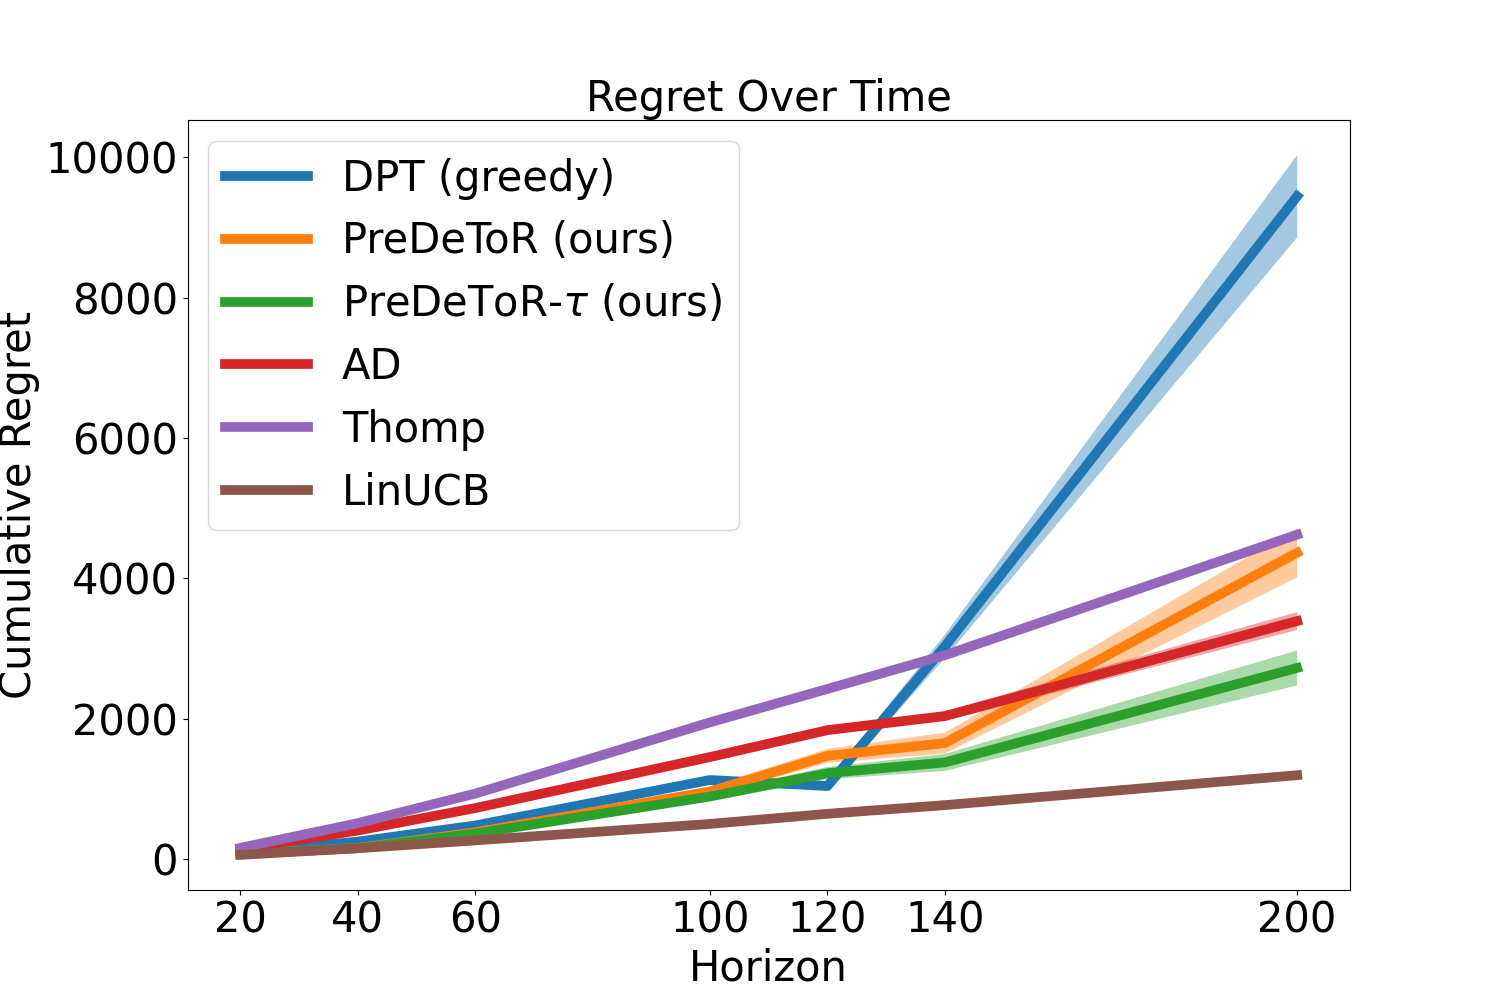
\includegraphics[scale = 0.13]{img/Neurips/horizon/horizon_fig.png} \label{fig:hor-inc}}
% \end{tabular}
% \vspace*{-1em}
% \caption{Experiment with increasing horizon. The y-axis shows the cumulative regret.}
% \label{fig:expt-horizon}
% \vspace{-0.7em}
% \end{figure}

\begin{figure}[!hbt]
\centering
\begin{subfigure}[b]{0.32\textwidth}
   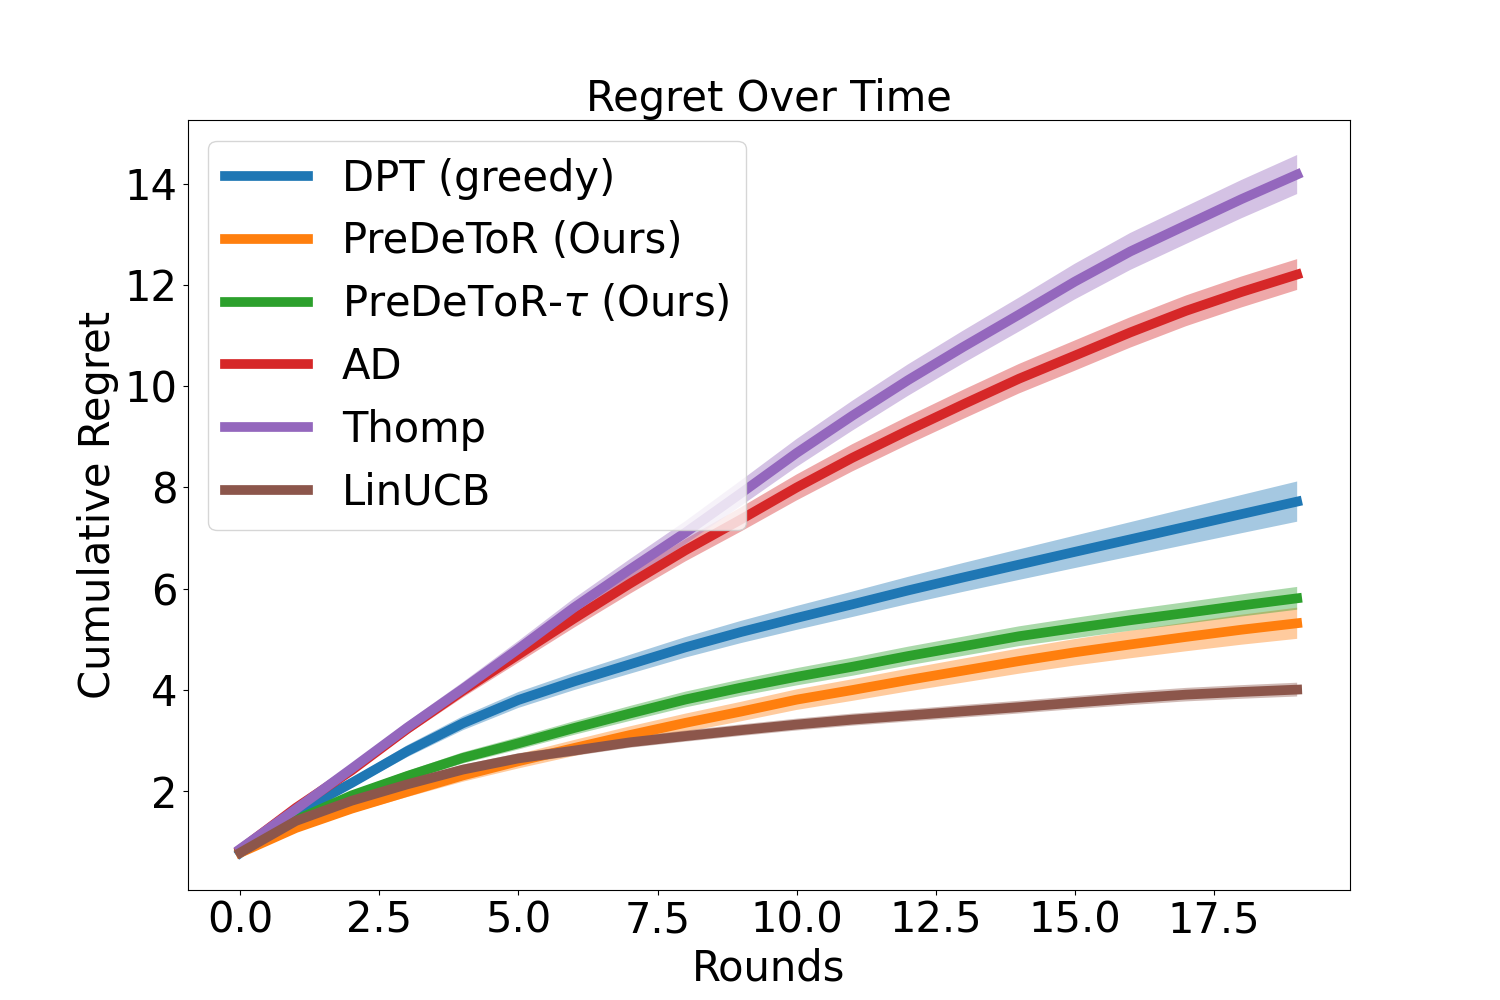
\includegraphics[scale=0.13]{img/Neurips/horizon/lin_H20_lr0.00015_do0_embd32_layer4_head4_envs150080_hists1_samples1_var0.3_cov0.0_H20_d20_lind5_seed1_testcov0.0_hor20.pkl.png}
   \caption{Horizon $20$}
   \label{fig:hor-20}
\end{subfigure}%
\begin{subfigure}[b]{0.32\textwidth}
   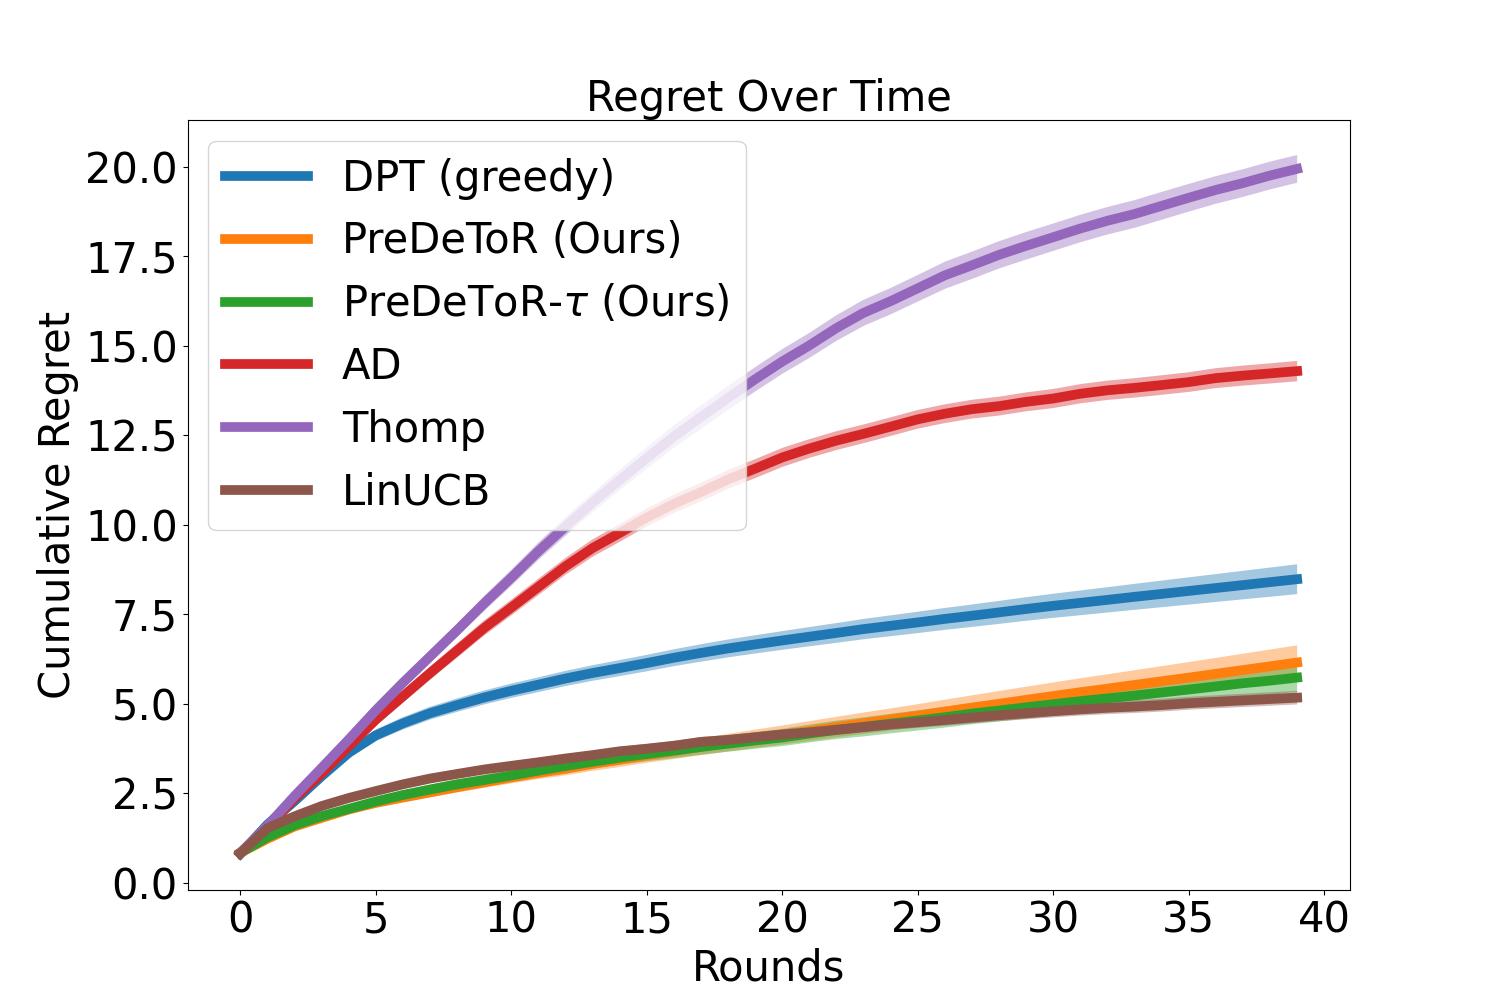
\includegraphics[scale=0.13]{img/Neurips/horizon/lin_H40_lr0.00015_do0_embd32_layer4_head4_envs150080_hists1_samples1_var0.3_cov0.0_H40_d20_lind5_seed1_testcov0.0_hor40.pkl.png}
   \caption{Horizon $40$}
   \label{fig:hor-40}
\end{subfigure}%
\begin{subfigure}[b]{0.32\textwidth}
   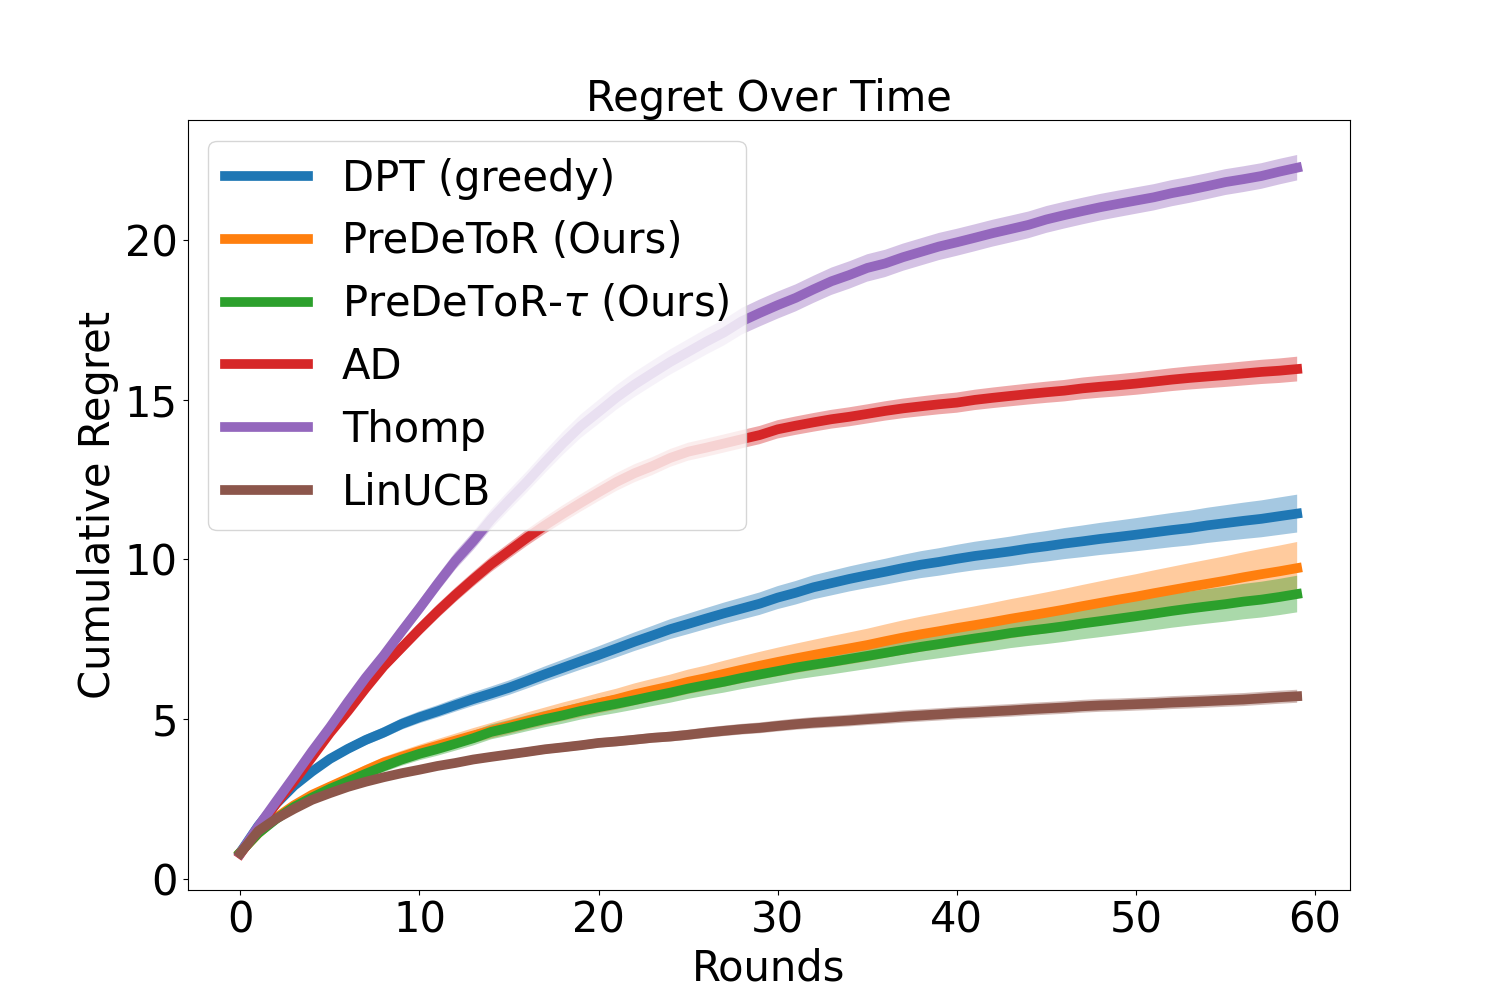
\includegraphics[scale=0.13]{img/Neurips/horizon/lin_H60_lr0.00015_do0_embd32_layer4_head4_envs150080_hists1_samples1_var0.3_cov0.0_H60_d20_lind5_seed1_testcov0.0_hor60.pkl.png}
   \caption{Horizon $60$}
   \label{fig:hor-60}
\end{subfigure}

\begin{subfigure}[b]{0.32\textwidth}
   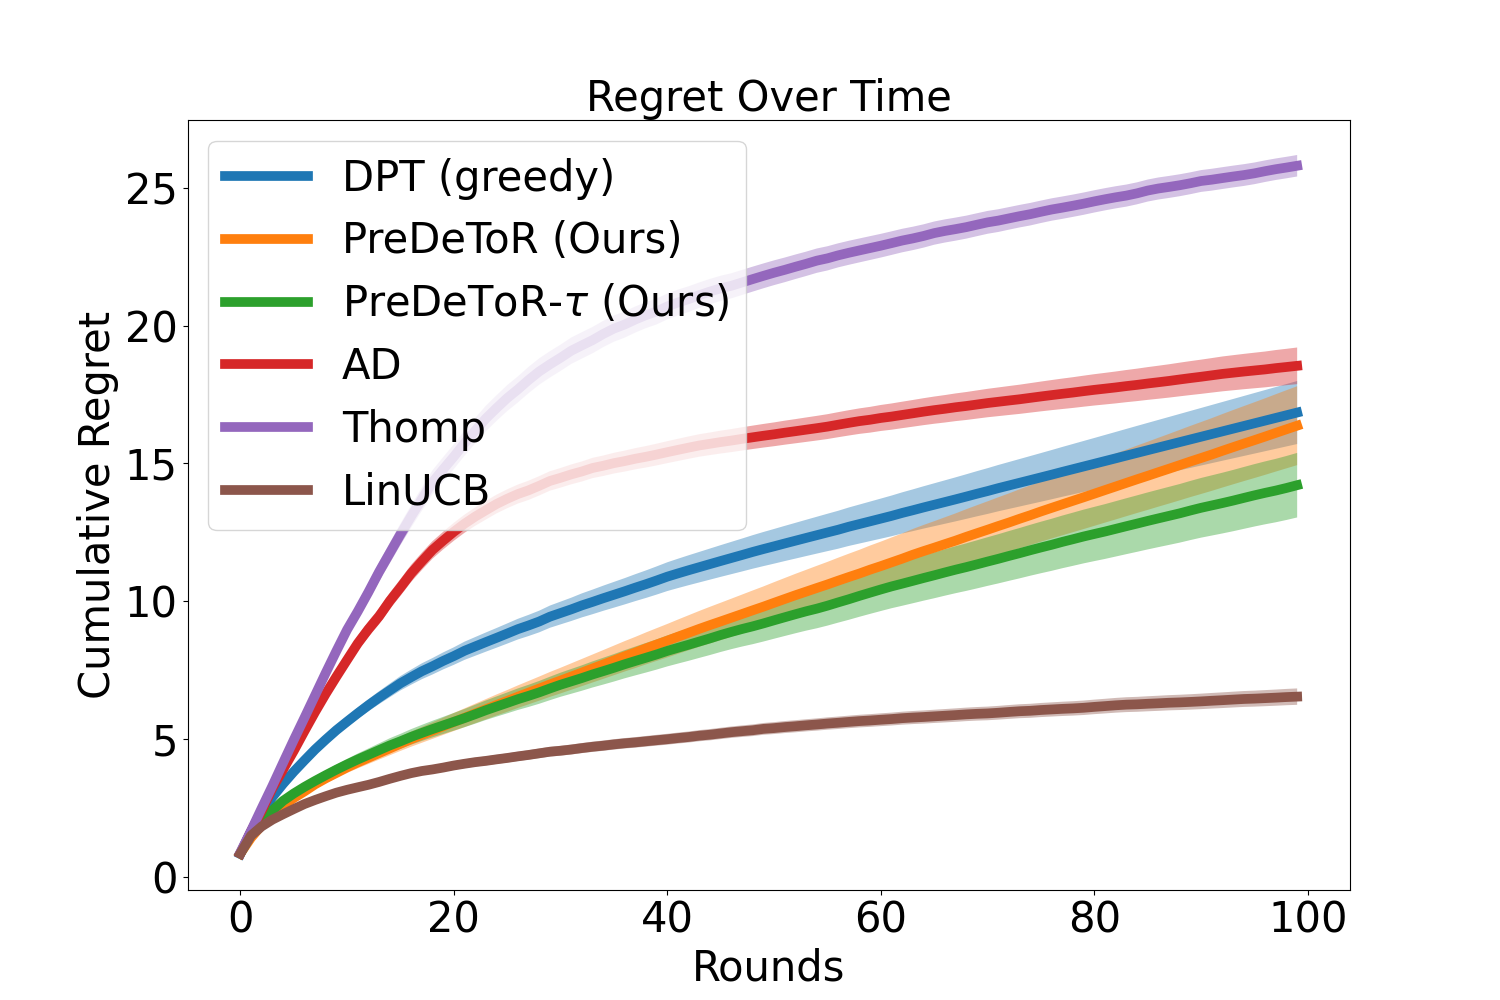
\includegraphics[scale=0.13]{img/Neurips/horizon/lin_H100_lr0.00015_do0_embd32_layer4_head4_envs150080_hists1_samples1_var0.3_cov0.0_H100_d20_lind5_seed1_testcov0.0_hor100.pkl.png}
   \caption{Horizon $100$}
   \label{fig:hor-100}
\end{subfigure}%
\begin{subfigure}[b]{0.32\textwidth}
   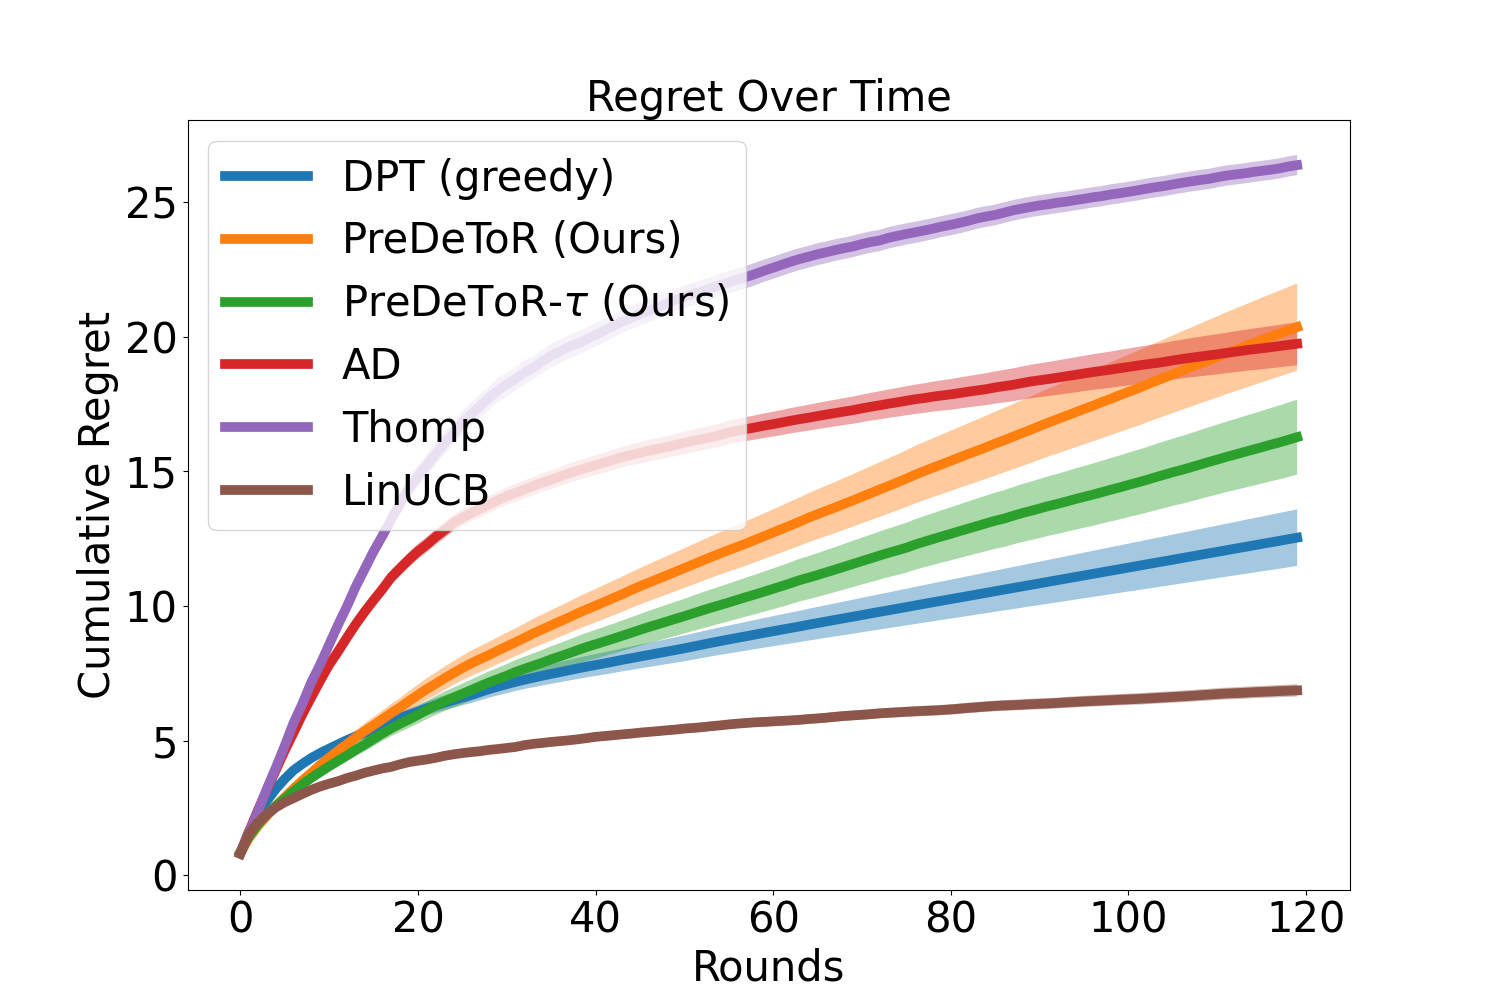
\includegraphics[scale=0.13]{img/Neurips/horizon/lin_H120_lr0.00015_do0_embd32_layer4_head4_envs150080_hists1_samples1_var0.3_cov0.0_H120_d20_lind5_seed1_testcov0.0_hor120.pkl.png}
   \caption{Horizon $120$}
   \label{fig:hor-120}
\end{subfigure}%
\begin{subfigure}[b]{0.32\textwidth}
   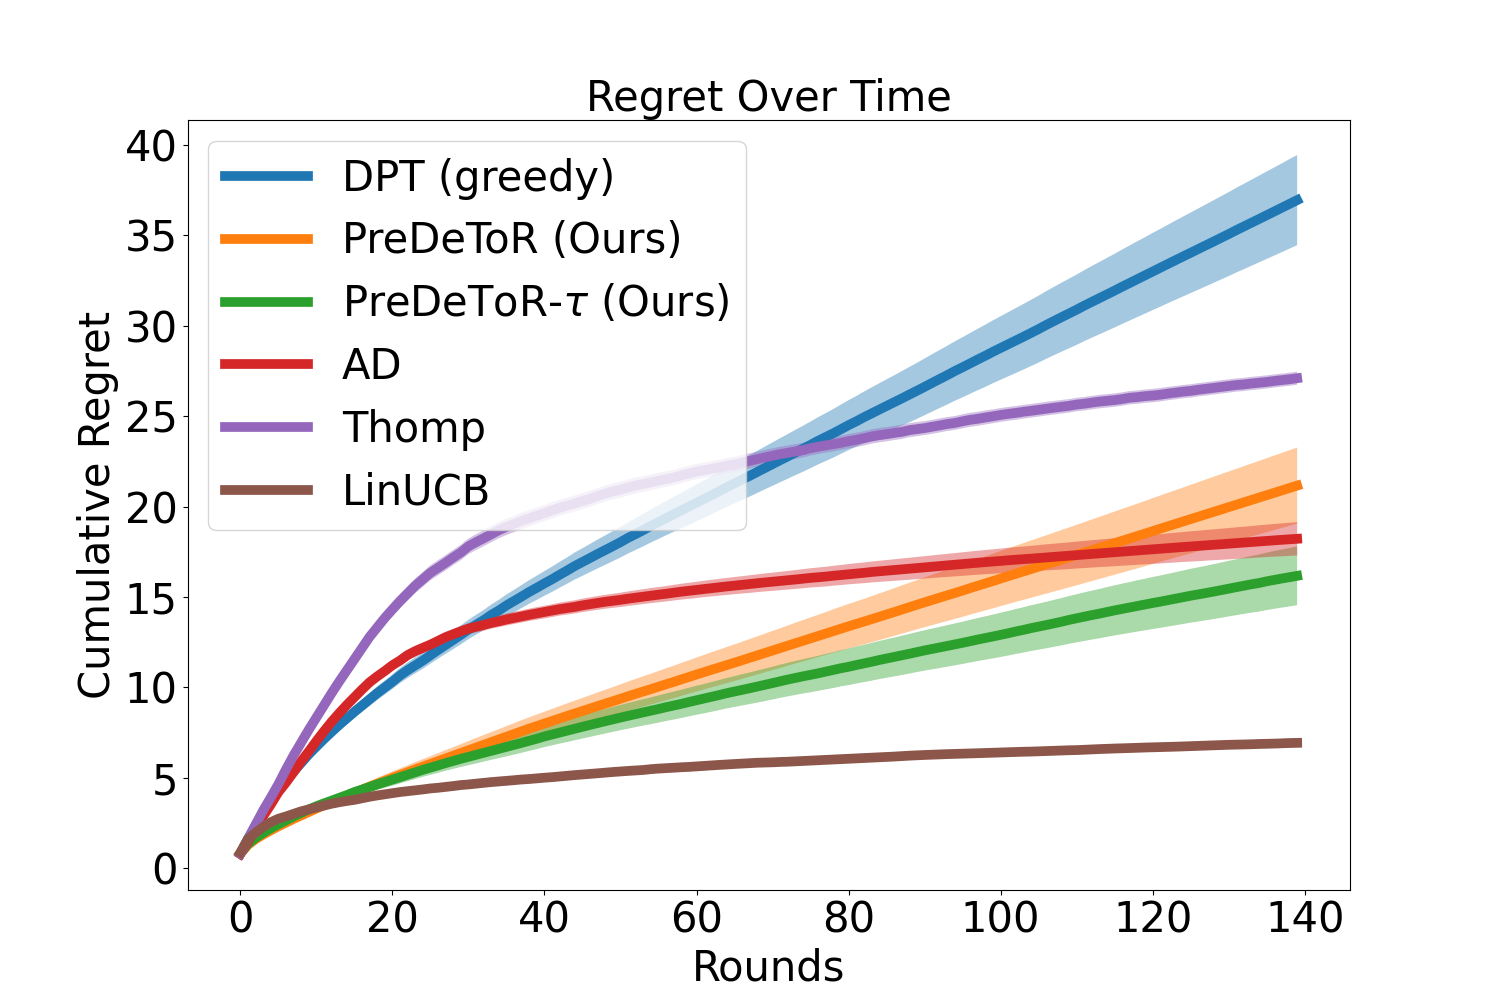
\includegraphics[scale=0.13]{img/Neurips/horizon/lin_H140_lr0.00015_do0_embd32_layer4_head4_envs150080_hists1_samples1_var0.3_cov0.0_H140_d20_lind5_seed1_testcov0.0_hor140.pkl.png}
   \caption{Horizon $140$}
   \label{fig:hor-140}
\end{subfigure}

\begin{subfigure}[b]{0.48\textwidth}
   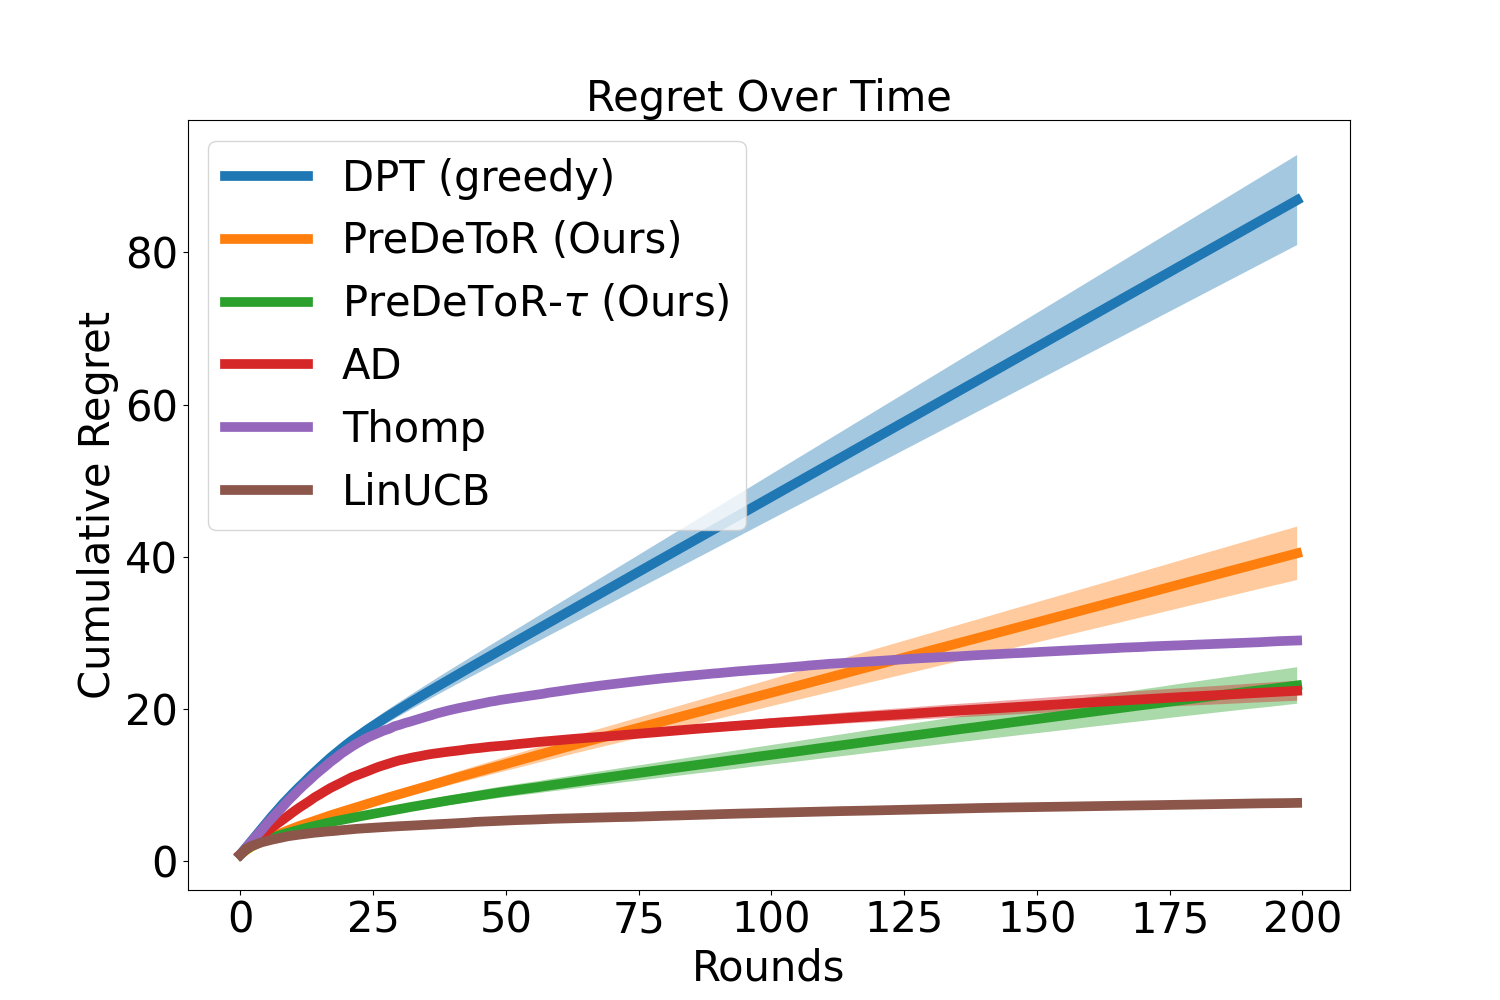
\includegraphics[scale=0.13]{img/Neurips/horizon/lin_H200_lr0.00015_do0_embd32_layer4_head4_envs150080_hists1_samples1_var0.3_cov0.0_H200_d20_lind5_seed1_testcov0.0_hor200.pkl.png}
   \caption{Horizon $200$}
   \label{fig:hor-200}
\end{subfigure}%
\begin{subfigure}[b]{0.48\textwidth}
   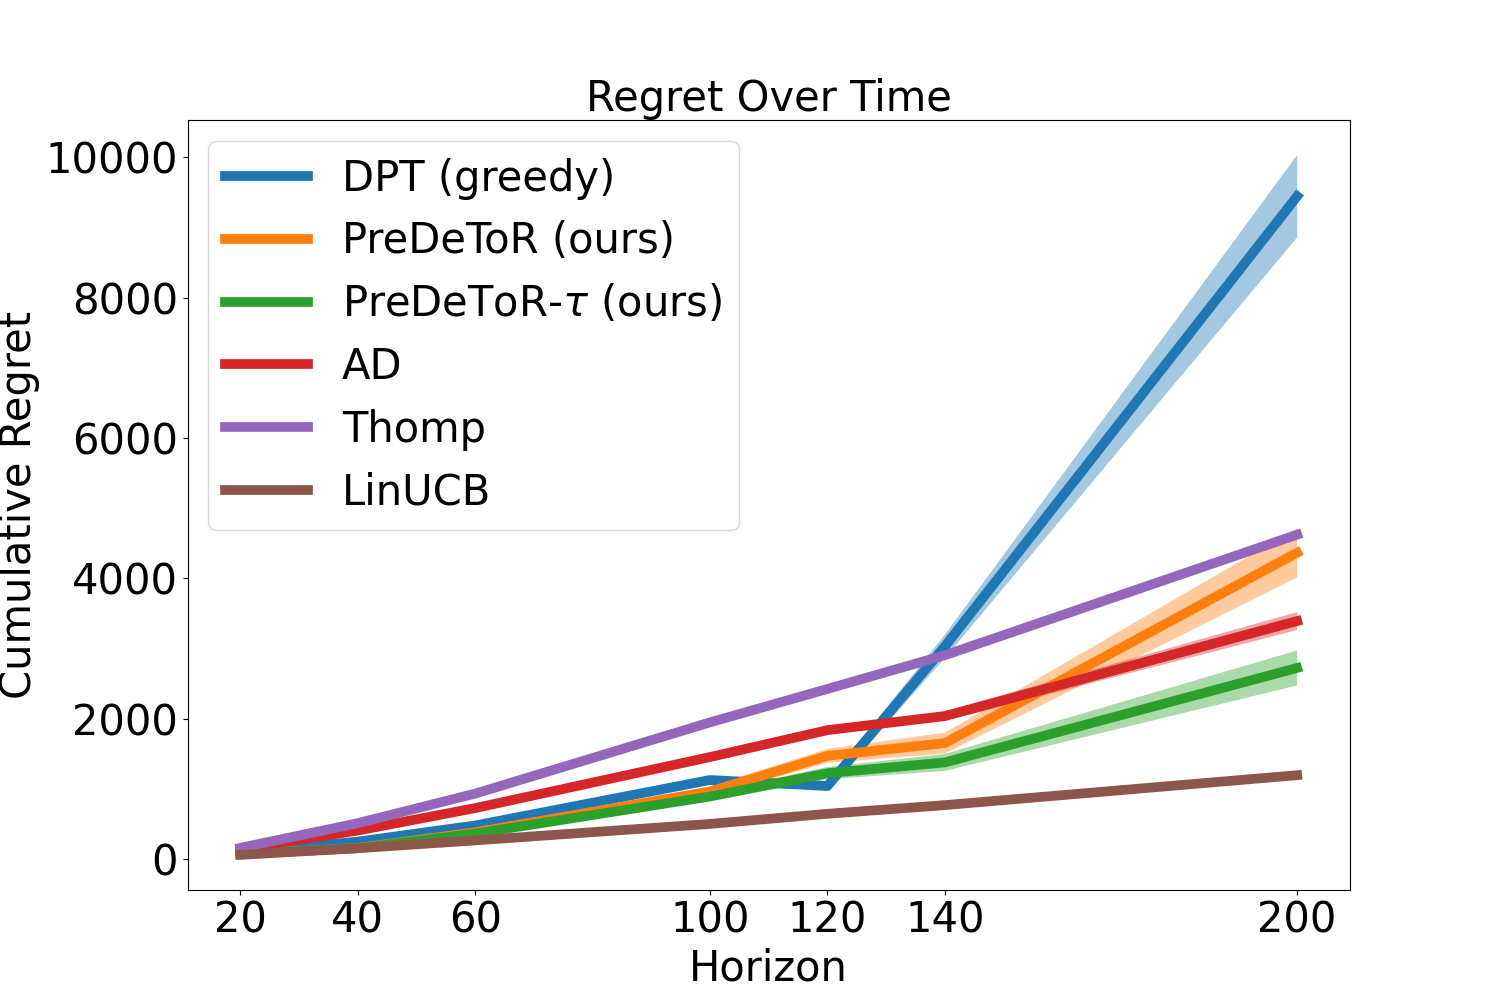
\includegraphics[scale=0.13]{img/Neurips/horizon/horizon_fig.png}
   \caption{Increasing Horizon}
   \label{fig:hor-inc}
\end{subfigure}
\vspace*{-1em}
\caption{Experiment with increasing horizon. The y-axis shows the cumulative regret.}
\label{fig:expt-horizon}
\vspace{-0.7em}
\end{figure}


\textbf{Experimental Result:} We observe these outcomes in \Cref{fig:expt-horizon}. In \Cref{fig:expt-horizon} we show the linear bandit setting for $\Mpr =  150000$, $\Mts = 200$, $A=20$, $n=\{20, 40, 60, 100, 120, 140, 200\}$ and $d=5$. 
%
%
Again, the demonstrator $\pi^w$ is the \ts\ algorithm. We observe that \pred\ (\gt) has lower cumulative regret than \dptg, and \ad. Note that for any task $m$ for the horizon $20$ the \ts\ will be able to sample all the actions at most once.
% Moreover \pred\ matches the performance of \linucb. 
%
%The weak performance of \dptg\ can be attributed to both short horizons and the inability to estimate the optimal action for such a short horizon $H < A$. 
%
%Note that for this small horizon setting the \dptg\ does not have a good estimation of $\widehat{a}_{m,*}$ which results in a poor prediction of optimal action $\widehat{a}_{m,t,*}$. 
% This results in higher regret. 
Observe from \Cref{fig:hor-20}, \ref{fig:hor-40}, \ref{fig:hor-60}, \Cref{fig:hor-100}, \ref{fig:hor-120}, \ref{fig:hor-140} and \ref{fig:hor-200} that \pred\ (\gt) is closer to \linucb\ and outperforms \ts\ which also shows that \pred\ (\gt) is learning the latent linear structure of the underlying tasks.
%
In \Cref{fig:hor-inc} we plot the regret of all the baselines with respect to the increasing horizon. Again we see that \pred\ (\gt) is closer to \linucb\ and outperforms \dptg, \ad\ and \ts.
%
% The training of \ad\ ensures that it does not outperform the demonstrator \ts.
%
This shows that \pred\ (\gt) is able to exploit the latent structure and reward correlation across the tasks for varying horizon length.


% the non-linear bandit setting for horizon $n=40$, $\Mpr =  200000$, $A=60$, $d=2$, and $|\Anc|=5$. The demonstrator $\pi^w$ is the \ts\ algorithm. Again we observe that \pred\ has lower cumulative regret than \dptg and it outperforms \linucb\ which fails to perform well in this non-linear setting due to its algorithmic design. 

% In the following two experiments, we test the limit of generalization of \pred\ by increasing the number of dimensions. In the linear setting experiment, we use $\Mpr =  400000$, $d=40$, $A=20$, and $H=15$. In the non-linear setting, we use $\Mpr =  300000$, $d=15$, $A=30$, and $H=15$. 
% %
% The corresponding results are shown in \Cref{fig:lim-dim-lin} and \Cref{fig:lim-nlm}. Observe that in the non-linear setting, the performance of \pred\ degrades and is almost similar to \dptg. This shows that as the number of dimensions increases and feedback is more complex, the ability of \pred\ to estimate the underlying latent structure and reward correlation also decreases.